\chapter{Dimensionality reduction}
\section{PCA}

It is obvious that less significant feature are better than a lot of irrelevant feature and also there is a problem of visualization with multivariate data. Moreover it is difficult to extract useful information from multivariate data.
So the problem of dimensionality reduction is about learn hypothesis map that reads representation of data point and transforms it to a set of features, the advantage are:
\begin{itemize}
    \item Capture the important information in a data set more efficiently than the original attributes
    \item Allow data to be more easily visualized
    \item Reduce overfitting
    \item Avoid curse of dimensionality
    \item Reduce amount of time and memory required by algorithms
    \item Help to eliminate irrelevant features or reduce noise
\end{itemize}

It was firstly introduced by y Pearson (1901) and Hotelling (1933) to describe the variation in a set of multivariate data in terms of a set of uncorrelated variables. The goal is reduce the feature, so starting from $n$ features we want to have $p$ new feature where $p$ << $n$ keeping more information as possible with the p variable that will be \textbf{uncorrelated}.

\begin{figure}[H]
    \centering
    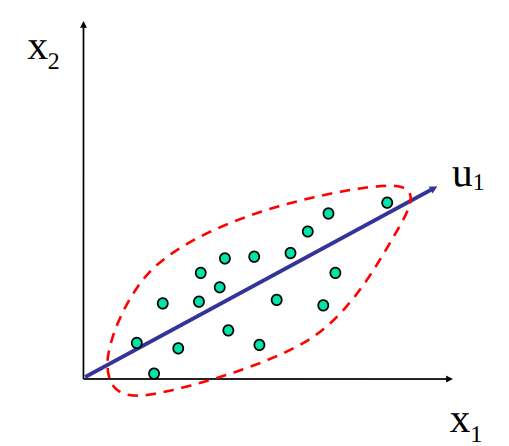
\includegraphics[scale=0.65]{images/DimRed/PCA1.png}
    \caption{Example of PCA}
    \label{fig:PCA}
\end{figure}

For example in the figure before we have in green the point with the feature $x_{1}$ and $x_{2}$ and we construct a function called $u_{1}$ to summarize this 2 features into 1; if we have bigger data we can choose between different $u$, but in this case the function have to be the one with the \textbf{largest variation}.

\begin{figure}[H]
    \centering
    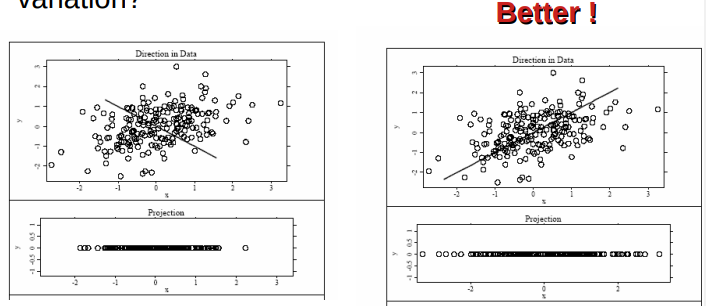
\includegraphics[scale=0.7]{images/DimRed/PCA2.png}
    \caption{Example of choosing the correct function $u$}
    \label{fig:enter-label}
\end{figure}

Principal component analysis is useful if there is some redundancy in variables or the data do not ‘span’ the whole of n dimensional space, because of this redundancy or space not covered, it is possible to
reduce the observed variables into a smaller number of principal components (artificial variables) 

It can be viewed as a rotation of the existing axes to new positions in the space defined by original variables and this new axes are orthogonal and represent the directions with maximum variability.
\begin{figure}[H]
    \centering
    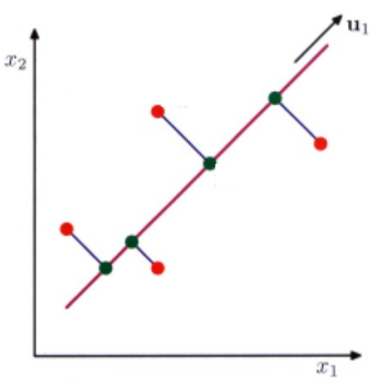
\includegraphics[scale=0.5]{images/DimRed/PCA3.png}
    \caption{PCA maximization}
    \label{fig:enter-label}
\end{figure}
\emph{\textbf{Definition}}: Principal component analysis seeks a space of lower dimensionality, known as the principal subspace and denoted by the magenta line, such that the orthogonal projection of the data points (red dots) onto this subspace \textbf{maximizes the variance of the projected points} (green dots). An alternative definition of PCA is based on \textbf{minimizing the sum-of-squares of the projection errors}, indicated by the blue lines.


A principal component can be defined as a linear combination of optimally-weighted observed variables and The number of components that can be extracted in a principal component analysis is equal to the number of observed variables. Oftenn only the first few components account for meaningful amounts of variance $(p<n)$. When the analysis is complete, the resulting components will display varying degrees of correlation with the observed variables, but are \textbf{completely uncorrelated} with one another

\subsection{Math part}
\paragraph{Single attribute}
With a single feature the calculus of the variance is very simple because the variance is only the power of 2 of the standard deviation
\begin{center}
    $variance = sd^2$\\
    $sd = \sqrt{\dfrac{1}{m-1} \sum\limits_{i=1}^m (x_i - \overline{x})^2}$ \\
    $s^2 = \dfrac{1}{m-1} \sum\limits_{i=1}^m (x_i - \overline{x})^2$
\end{center}
\paragraph{Two attributes}
Covariance: measures the correlation between x and y
\begin{center}
    $cov(x,y) = \dfrac{1}{m-1} \sum\limits_{i=1}^m (x_i - \overline{x}) (y_i - \overline{y})$
\end{center}
\begin{itemize}
    \item cov(x,y)=0: independent, we want to reach that
    \item cov(x,y)>0: move same direction
    \item cov(x,y)<0: move opposite directions
\end{itemize}
\paragraph{More than two attributes}
To have all the other number of feature we can create a covariance matrix like in the next figure, that matrix contains covariance values between all possible dimensions.
\begin{figure}[H]
    \centering
    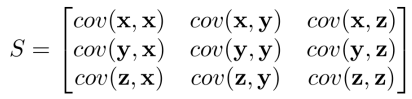
\includegraphics{images/DimRed/PCA4.png}
    \caption{Example of covariance matrix}
    \label{fig:enter-label}
\end{figure}

\begin{center}
    Sample covariance matrix S (n x n) of X (m x n) can be written as:\\
    $ S = \dfrac{1}{m-1} \sum\limits_{i=1}^m (X - \overline{X})^t (X - \overline{X})$\\
    where $\overline{X}$ (m x n) is the matrix of the mean attributes (all m rows are equal, corresponding to the mean of all m rows of X)
\end{center}
Before proceeding with something useful for the PCA there are some mathematical stuff to know.
\paragraph{Eigenvalues and eigenvector}
Vectors u having same direction as Au are called eigenvectors of A (A is an n by n matrix),  In the equation Au=$\lambda$u, $\lambda$ is called an eigenvalue of A.\\
$\begin{bmatrix}
    2 & 3 \\
    2 & 1 
\end{bmatrix}
=
\begin{bmatrix}
    3\\
    2
\end{bmatrix}
= 4
\begin{bmatrix}
    3\\
    2
\end{bmatrix}
$\\\\
Then we can look to some matrix formulas:
\begin{center}
    $(A^t)^t =A $\\
    $P^{-1} = P^t$\\
    $(A \pm B) =A^t \pm B^t$\\  
    $(cA)^t =cA^t$\\
    $(AB)^t= B^t A^t$
\end{center}

Now we can start talking about the orthogonality and orthonormality. 
Two vectors $u_1$ and $u_2$ (n x 1) for which $u_1^t u_2=0$ holds are said to be orthogonal, the idea is that to be orthogonal in the image they have to be perpendicular.
The feature transformation is a change of the basis with orthonormal vectors so we have to find orthonormal P (n x n) such that $X'= XP^t$ with cov(X') diagonalized (\textbf{variables uncorrelated}). The (first p) rows of P are the principal components of X.
 
To find P with cov(X') diagonalized (diagonal equal to 0):
\begin{center}
    $ cov(X') = \dfrac{1}{m-1} (X')^t (X')$  if X' has zero means so we can just cancel $\overline{X}$\\
    = $\frac{1}{m-1} (X P^t)^t (XP^t)$ \\
    = $\frac{1}{m-1} X^t P X P^t $ = $\frac{1}{m-1} P(X^t X )P^t $ = $\frac{1}{m-1} PAP^t$
\end{center}

That $A =X^t X$ is symmetric (n x n), therefore there is a matrix E of eigenvectors of A and a diagonal Matrix called D such that $A = EDE^t$. Now we define P to be the transpose of the matrix E of eigenvectors $P:= E^t$ then we can write A as $ A = P^t D P $. Remember that $E = (u_1, u_2, u_3, \dots)$ as column, all the possible eigenvectors.

With this definition we substitute the values:
\begin{center}
    $ cov(X') = \dfrac{1}{m-1} PAP^t = \dfrac{1}{m-1} PP^t D PP^t= \dfrac{1}{m-1}D =S'$
\end{center}

If we define P as the transpose eigenvector matrix will have as a result a Diagonal (D) covariance matrix with the diagonal equal to 1 and 0 in any other.

$S' = cov(X') =
\begin{bmatrix}
    1 & 0 & 0 \\
    0 & 1 & 0 \\
    0 & 0 & 1 \\
\end{bmatrix}$

P diagonalized cov(X') where P is the transpose of the matrix of eigenvectors of $ A=XX^t$ and the principal components  of X are the eigenvectors of $A=X^tX$, moreover the $i_{th} $ diagonal value of cov(X') is the variance of X' along $u_i$ (along the $i_{th}$ principal component, the $i_{th}$ row of P).

$S' = \begin{bmatrix}
    \sigma_1 & 0 & 0 \\
    0 & \sigma_2 & 0 \\
    0 & 0 & \sigma_3 \\
\end{bmatrix}
    \\
    \sigma_1 = cov(x_1,x_1) = var(x_1)
$

Essentially, we need  to take the covariance`matrix of the original matrix X and compute:
\begin{enumerate}
    \item Eigenvalues: explained variance
    \item Eigenvectors: new axis, principal components
\end{enumerate}

In the diagonal matrix we have to take the maximum eigenvalues, that has the maximum variance, and it will be the first component or Principal Component PC1. The second, instead, have the direction with maximum variation left in data orthogonal to PC1. The eigenvector corresponding to the second largest eigenvalue.

\subsubsection{Steps of PCA}
\begin{enumerate}
    \item Let $\overline{X} $ be the mean matrix (all rows are equal, corresponding to the mean of all rows)
    \item Adjust the original data by the mean $X-\overline{X}$
    \item Compute the covariance matrix S of X: $ S = \dfrac{1}{m-1} \sum\limits_{i=1}^m (X - \overline{X})^t (X - \overline{X})$
    \item Find the eigenvectors and eigenvalues of S
    \item For matrix S, vectors u (=column vector) having same direction as Su, with factor $\lambda$
    \item Eigenvalues $\lambda_i$ corresponds to variance on each component i=1,...,n
    \item Thus, sort by $\lambda_i$
    \item Take the first p eigenvectors $u_i$; where p is the number of top eigenvalues. Form matrix P
    \item These are the directions with the largest variance
    \item Project the original data: $XP^t$
\end{enumerate}

There is a correlation between Eigenvalues and the Variance because Eigenvalues $\lambda_i$ are used for calculation of [\% of total variance] (Vi) for each component i: $ V_i = 100 \dfrac{\lambda_i}{\sum\limits_{j=1}^n \lambda_j} $ and if the data are \textbf{standardized} $\sum\limits_{j=1}^n \lambda_j = n $

\begin{figure}[H]
    \begin{subfigure}{.4\textwidth}
        \centering
        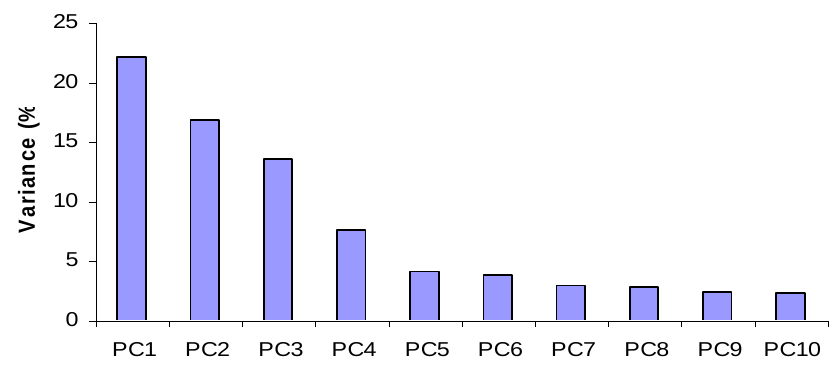
\includegraphics[width=1\linewidth]{images/DimRed/PCA5.png}
        \caption{Visual representation of Variance}
        \label{fig:sub1}
    \end{subfigure}
    \begin{subfigure}{.5 \textwidth}
        \centering
        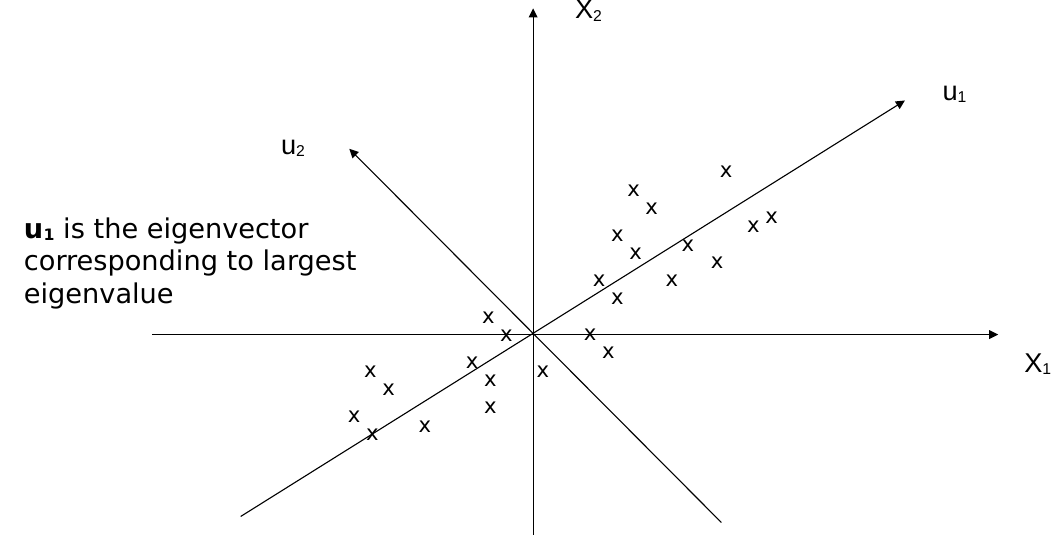
\includegraphics[width=1\linewidth]{images/DimRed/PCA6.png}
        \caption{New basis with $u_1$ and $ u_2$}
        \label{fig:sub1}
    \end{subfigure}
    \caption{Eigenvalues and Eigenvectors}
\end{figure}

\subsubsection{Properties}
 The properties of the principal components are:
 \begin{itemize}
     \item  linear combinations of the original variables
     \item  uncorrelated with each other
     \item capture as much of the original variance as possible
 \end{itemize}

Another important things to considered is the criteria of when to stop the PCA (choosing the p).
\begin{enumerate}
    \item Kaiser criterion: keep PCs with eigenvalues > 1 (variance explained more than a single original variable)
    \item Proportion of variance explained: enough PCs to have cumulative variance explained that is larger than a threshold (e.g., 66\%)
    \item  Elbow method: start of the bend in the line (point of inflexion) indicate how many components are retained
\end{enumerate}
\begin{figure}[H]
    \centering
    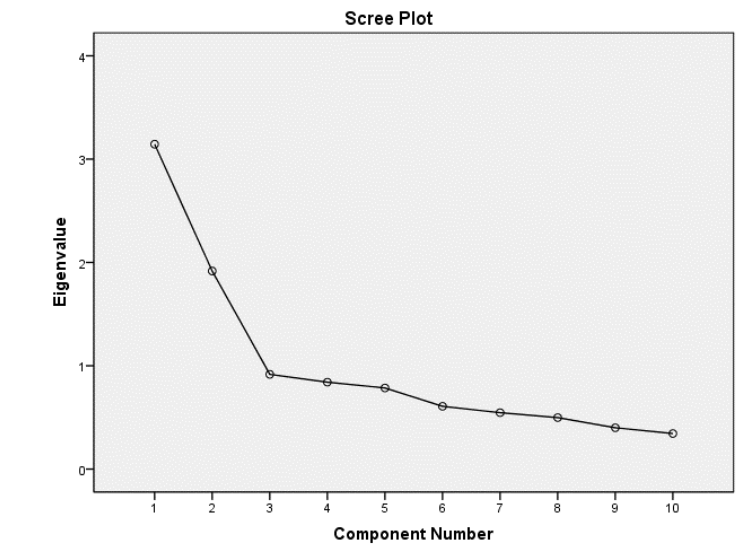
\includegraphics[scale=0.5]{images/DimRed/PCA7.png}
    \caption{Example of PCA Elbow method}
    \label{fig:enter-label}
\end{figure}

\subsection{Proof of eigenvalues - maximize variance}
Assuming $X \in R^{m \times n}$ as the data and $x_{i,j}$ as one value.
We want to find a number of feature $p << n$ that describe the entire data in an efficient way (best variance possible). In the example with $p=1$ we want to have only one feature and 1 vector and trying to maximize the variance. 
So the vector called $u_1 \in R^{1 \times n}$. The projection on the data has to be $ x_i \times u_1^T$ on a single dimension.\\
It is time to calculate the \textbf{mean projected data} as $ \overline{x} \times u_1^T $ and then the variance $ \frac{1}{m-1} \sum\limits_{i=1}^m (x_i \times u_1^T - \overline{x} \times u_1^T)^2$. The aim is to maximize this function.\\

max $ \frac{1}{m-1} \sum\limits_{i=1}^m (x_i \times u_1^T - \overline{x} \times u_1^T)^2$ =  max $(u_1 S u_1^T)$ with S equal to the covariance of the original matrix, but max $(u_1 S u_1^T)$ derivative tend to infinite because $|| u_1||$ tend to infinite. We add the constraint $|| u_1||$ that allows $u_1 u_1^T =1$.\\
$max_{u_1} (u_1 S u_1^T + \lambda (1 - u_1 u_1^T  ) $ with the second part that is a penalty to not consider the constrain. We do the derivative of that function in respect of $u_1$ as $ 2 S U_1^T - \lambda 2u_1^T = 0 $. NB = 0 because it is the results we want in order to maximize.\\
We obtain $S u_1^T = \lambda u_1^T $ that is the eigenvalue and eigenvector formula with $u_1$ eigenvector and $\lambda$ eigenvalue. Left multiplying by $u_1$ we obtain $u_1 S u_1^T = u_1 \lambda u_1^T $ and then we can change $u_1 \lambda u_1^T \rightarrow \lambda u_1 u_1^T$ , since $ u_1 u_1^T = 1$ we finally have $u_1 S u_1^T = \lambda$.

So in the left we have the variance of the projected data. So to maximize the variance we have to choose the maximum eigenvalue.




\section{Non linear dimensionality reduction}
Not all the data are linear so PCA don't work on all possibility.
\textbf{Kernel PCA} transform points on different feature space and then apply PCA and the results are not in a linear space.
\textbf{T-SNE} frequently used only for visualization, function with probability distribution on n-dimensional space and thern we take a similar probability distribution on lower p-dimensional space. This have to be performed iteratively until the Kullback-Leibler divergence between  distribution is minimized.